\chapter{Применение программы PCLAB при исследовании производительности ЭВМ}

Программа PCLAB предназначена для исследования производительности x86 совместимых ЭВМ c IA32 архитектурой, работающих под управлением операционной системы Windows (версий 95 и старше).

Процесс сбора и анализа экспериментальных данных в PCLAB основан на процедуре профилировки критического кода, т.е. в измерении времени его обработки центральным процессорным устройством. Для измерения времени работы циклов в PCLAB используется следующая методика:

\begin{itemize}
	\item длительность обработки участка профилируемой программы характеризуется изменением величины счетчика тактов процессора, произошедшим за время его работы;
	\item для предотвращения влияния соседних участков кода на результаты измерений, перед началом замера и после его окончания необходимо выдать команду упорядоченного
выполнения CPUID, препятствующую переупорядочиванию потока команд на конвейере процессора;
	\item замеры количества тактов процессора необходимо повторить несколько раз;
	\item взаимное влияние последовательных повторов экспериментального участка программы исключается благодаря очищению кэш-памяти и буферов процессора;
	\item часть граничных результатов отбрасывается (как наибольших, так и наименьших). По оставшимся результатам замеров определяется средняя величина.
\end{itemize}

\chapter{Идентификация процессора}

Из выполнения команды идентификации процессора CPUID получены характеристики процессора, показанные на рисунке \ref{img:params}.

\begin{figure}[H]
	\begin{center}
		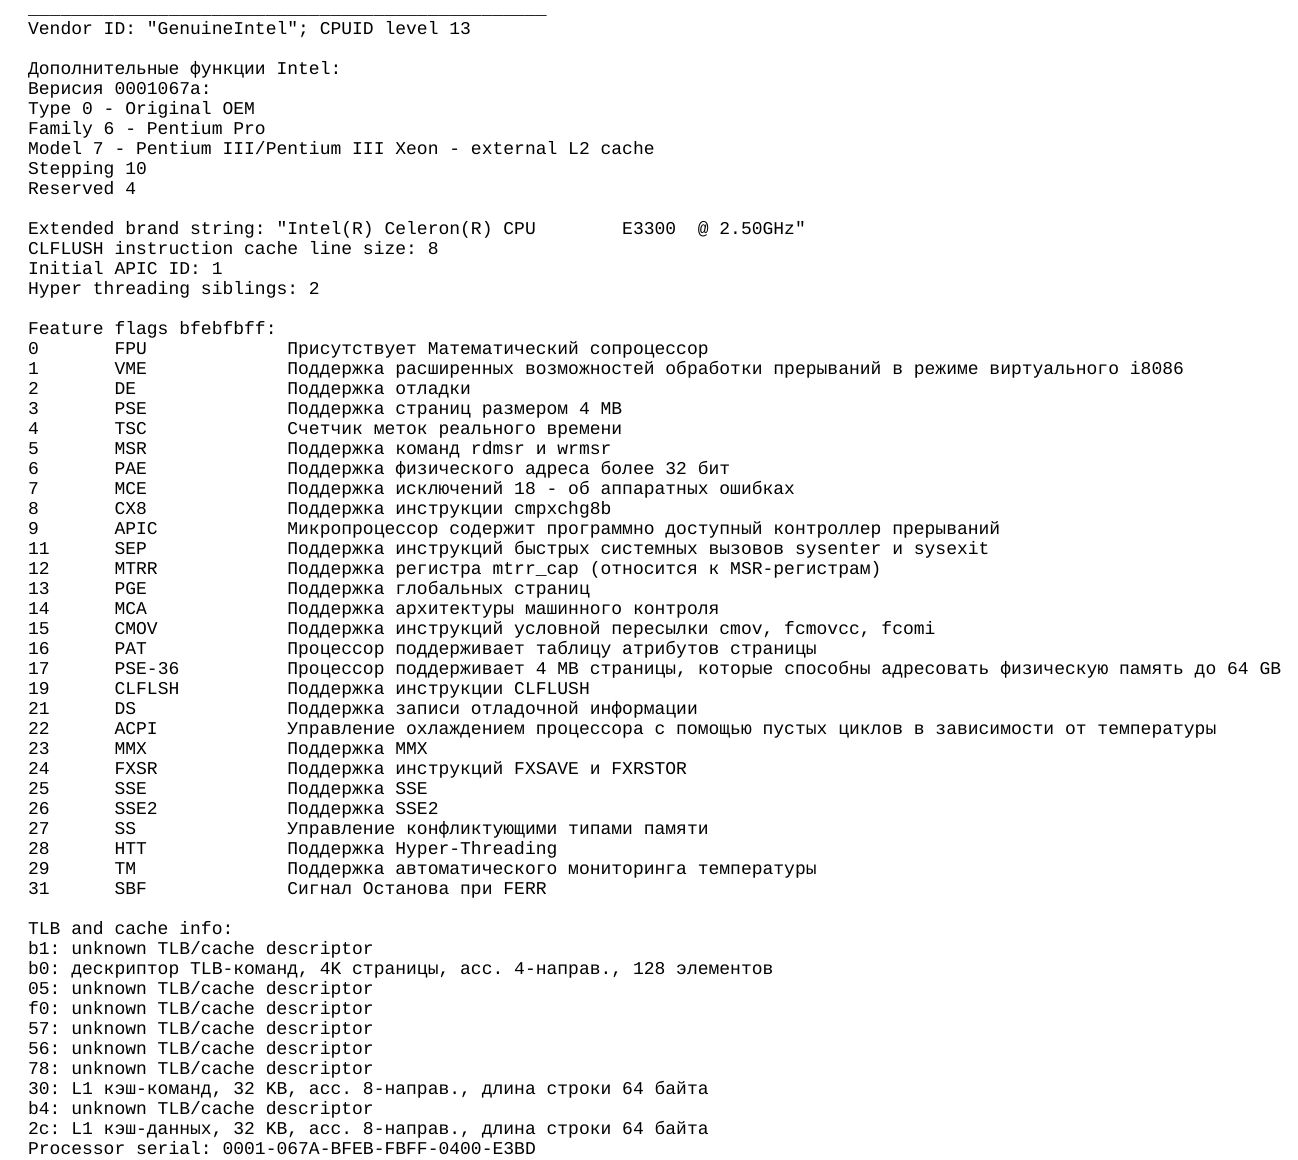
\includegraphics[scale=0.3]{img/params.png}
	\end{center}
	\captionsetup{justification=centering}
	\caption{Характеристики процессора}
	\label{img:params}
\end{figure}

Таким образом, размер линейки кэш-памяти верхнего уровня микропроцессора равен 8, объем физической памяти микропроцессора равен 2 ГБ.

\chapter{Эксперимент «Исследование расслоения динамической памяти»}

Цель эксперимента заключается в определении способа трансляции физического адреса, используемого при обращении к динамической памяти.

\section{Исходные данные}

\begin{itemize}
	\item размер линейки кэш-памяти верхнего уровня;
	\item объем физической памяти.
\end{itemize}

\section{Настраиваемые параметры}

\begin{itemize}
	\item максимальное расстояние между читаемыми блоками, равное 6;
	\item шаг увеличения расстояния между читаемыми 4-х байтовыми ячейками, равный 8;
	\item размер массива, равный 2.
\end{itemize}

\section{Графики полученных характеристик}

На рисунке \ref{img:delimitation} график показывает количество тактов работы алгоритма. Ось абсцисс отражает шаг приращения адреса читаемых данных. Ось ординат отображает количество тактов.

\begin{figure}[H]
	\begin{center}
		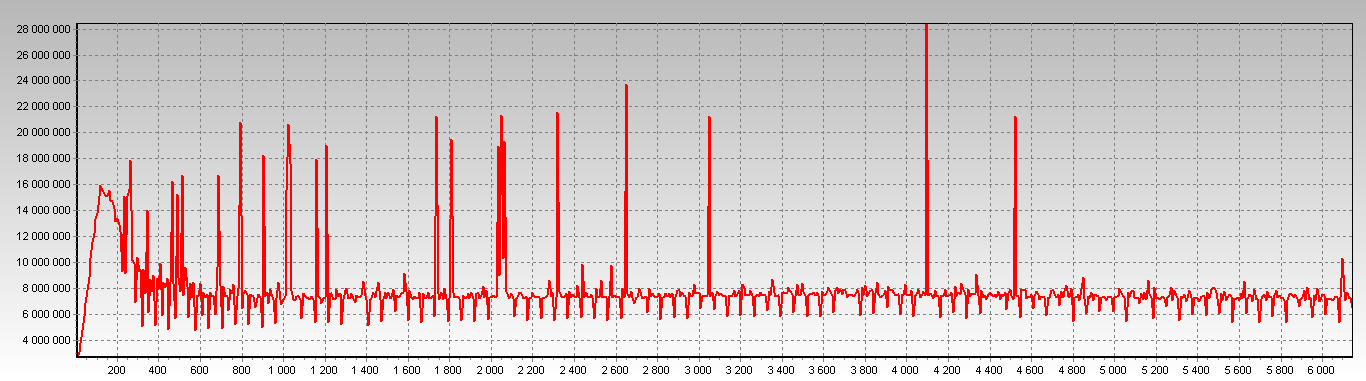
\includegraphics[scale=0.3]{img/delimitation.jpg}
	\end{center}
	\captionsetup{justification=centering}
	\caption{Исследование расслоения динамической памяти}
	\label{img:delimitation}
\end{figure}

\section{Результаты эксперимента}

В результате исследования расслоения динамической памяти были получены следующие параметры:

\begin{itemize}
	\item минимальный шаг чтения динамической памяти, при котором происходит постоянное обращение к одному и тому же банку, равный $T1 = 120$ Б.
	\item количество банков динамической памяти, равное $Б = 120(128) / 64 = 2(1.875)$; 
	\item расстояние между началом двух последовательных страниц одного банка, равное $T2 = 4096$ Б;
	\item размер одной страницы динамической памяти, равный $PC = 4096 / 2 = 2048$ Б;
	\item количество страниц в динамической памяти, равный $С =  4096 * 64 * 8 / (2048 * 2 * 64) = 8$.
\end{itemize}

\section{Вывод}

Оперативная память неоднородна, и для обращения к последовательно расположенным данным может потребоваться различное количество времени.

\chapter{Эксперимент «Сравнение эффективности ссылочных и векторных структур данных»}

Цель эксперимента заключается в оценке влияния зависимости команд по данным на эффективность вычислений.

\section{Настраиваемые параметры}

\begin{itemize}
	\item количество элементов в списке, равное 1;
	\item максимальная фрагментация списка, равная 256;
	\item шаг увеличения фрагментации, равный 4.
\end{itemize}

\section{Графики полученных характеристик}

На рисунке \ref{img:struct} красный график (верхний) показывает количество тактов работы алгоритма, использующего список. Зеленый график (нижний) показывает количество тактов работы алгоритма, использующего массив. Ось абсцисс отражает фрагментацию списка. Ось ординат отображает количество
тактов.

\begin{figure}[H]
	\begin{center}
		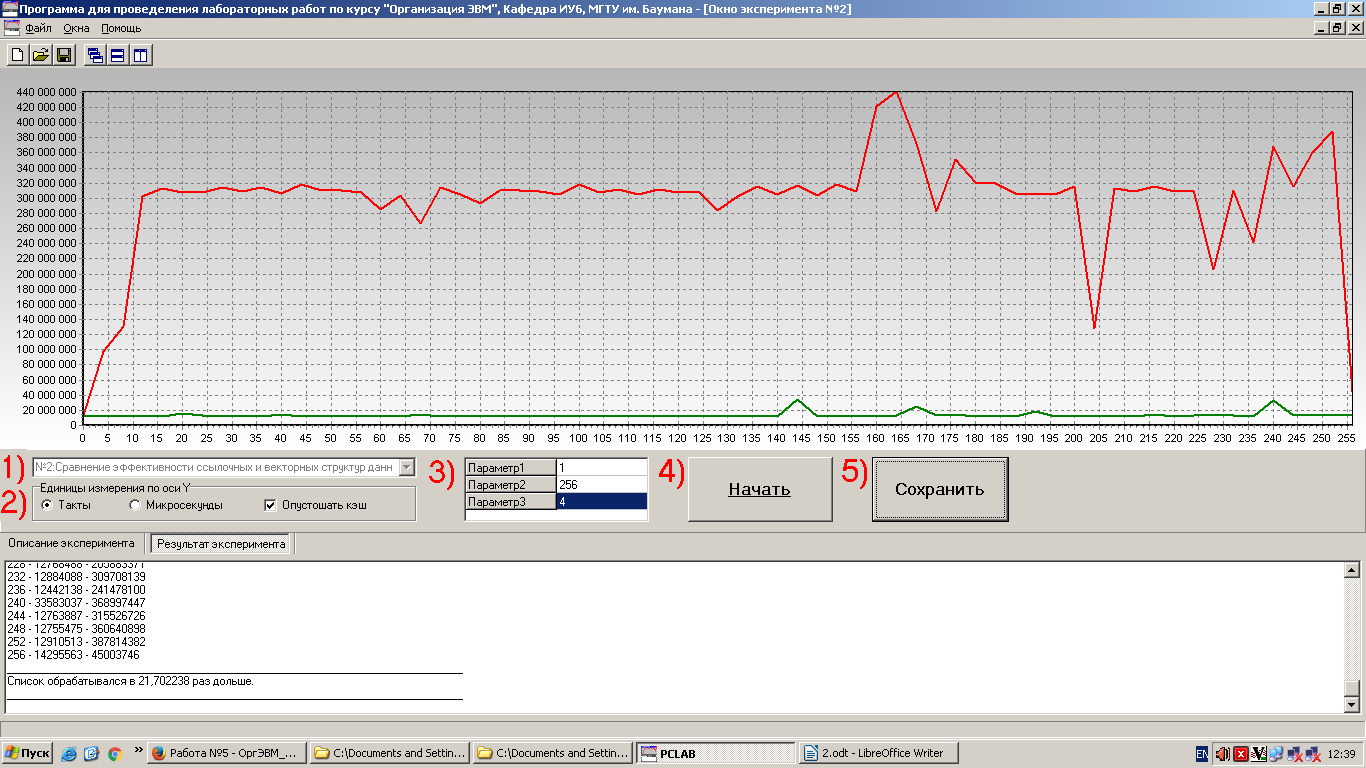
\includegraphics[scale=0.3]{img/struct.jpg}
	\end{center}
	\captionsetup{justification=centering}
	\caption{Исследование эффективности ссылочных и векторных структур}
	\label{img:struct}
\end{figure}

\section{Результаты эксперимента}

В результате исследования эффективности ссылочных и векторных структур, показанном на рисунке \ref{img:struct}, получено, что cписок обрабатывался в 21,702238 раз дольше.

\section{Вывод}

Использовать структуры данных необходимо с учетом технологического фактора определенной задачи.

\chapter{Эксперимент «Исследование эффективности программной предвыборки»}

Цель эксперимента заключается в выявлении способов ускорения
вычислений благодаря применению предвыборки данных.

\section{Исходные данные}

\begin{itemize}
	\item степень ассоциативности;
	\item размер TLB данных.
\end{itemize}

\section{Настраиваемые параметры}

\begin{itemize}
	\item шаг увеличения расстояния между читаемыми данными, равный 64;
	\item размер массива, равный 128.
\end{itemize}

\section{Графики полученных характеристик}

На рисунке \ref{img:effective} красный график (верхний с острыми пиками) показывает количество тактов работы алгоритма без предвыборки. Зеленый график (нижний без значимых пиков) показывает количество тактов работы алгоритма с использованием
предвыборки. Ось абсцисс отражает смещение читаемых данных от начала блока. Ось ординат отображает количество тактов.

\begin{figure}[H]
	\begin{center}
		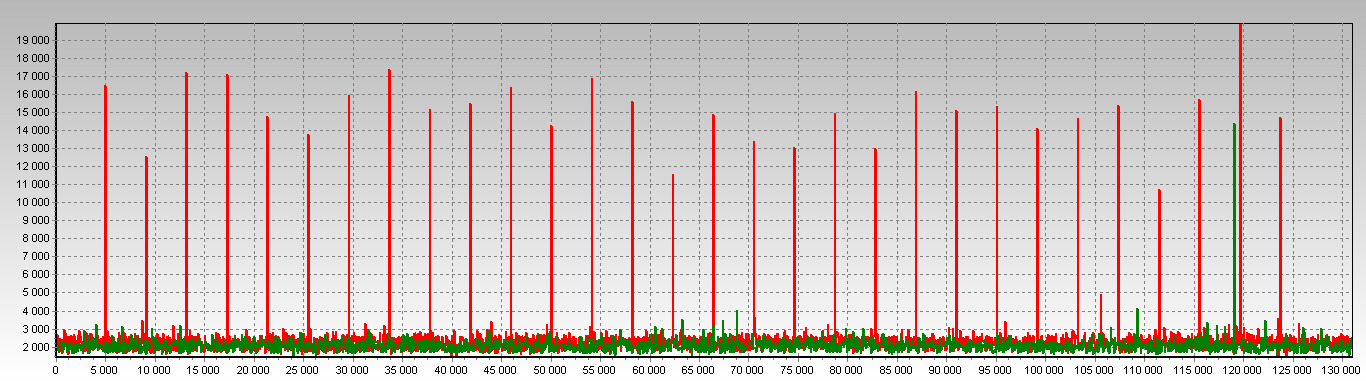
\includegraphics[scale=0.3]{img/effective.jpg}
	\end{center}
	\captionsetup{justification=centering}
	\caption{Исследование эффективности предвыборки}
	\label{img:effective}
\end{figure}

\section{Результаты эксперимента}

В результате исследования эффективности предвыборки, показанном на рисунке \ref{img:effective_result}, получено, что обработка без загрузки таблицы страниц в TLB производилась в 1,1726314 раз дольше.

\begin{figure}[H]
	\begin{center}
		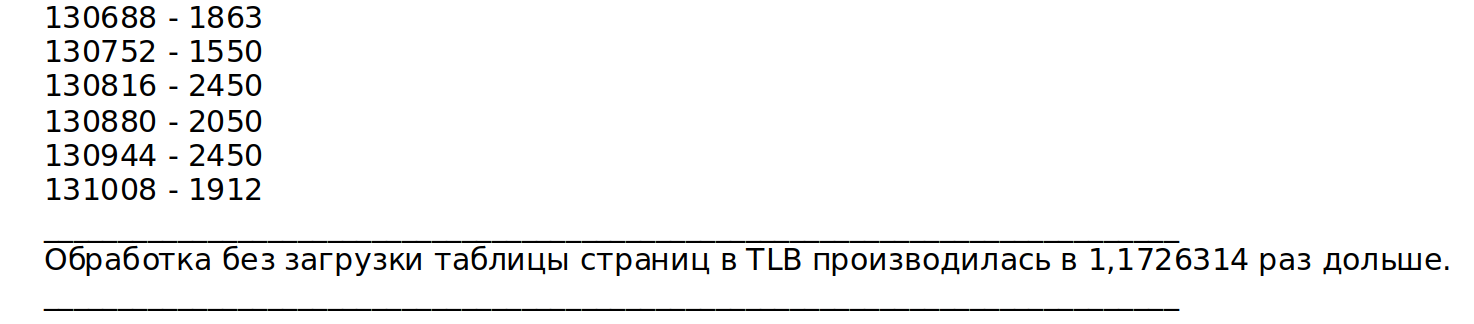
\includegraphics[scale=0.3]{img/effective_result.png}
	\end{center}
	\captionsetup{justification=centering}
	\caption{Результат исследования эффективности предвыборки}
	\label{img:effective_result}
\end{figure}

\section{Вывод}

За счет заблаговременной загрузки страниц в память можно ускорить время работы программы.

\chapter{Эксперимент «Исследование способов эффективного чтения оперативной памяти»}

Цель эксперимента заключается в исследовании возможности ускорения вычислений благодаря использованию структур данных, оптимизирующих механизм чтения оперативной памяти.

\section{Исходные данные}

\begin{itemize}
	\item адресное расстояние между банками памяти;
	\item размер буфера чтения.
\end{itemize}

\section{Настраиваемые параметры}

\begin{itemize}
	\item размер массива, равный 2;
	\item количество потоков данных, равное 64.
\end{itemize}

\section{Графики полученных характеристик}

На рисунке \ref{img:read} красный график (верхний) показывает количество тактов работы алгоритма, использующего неоптимизированную структуру. Зеленый график (нижний) показывает количество тактов работы алгоритма с использованием оптимизированной структуры. Ось абсцисс отражает сколичество одновременно обрабатываемых массивов. Ось ординат отображает количество тактов.

\begin{figure}[H]
	\begin{center}
		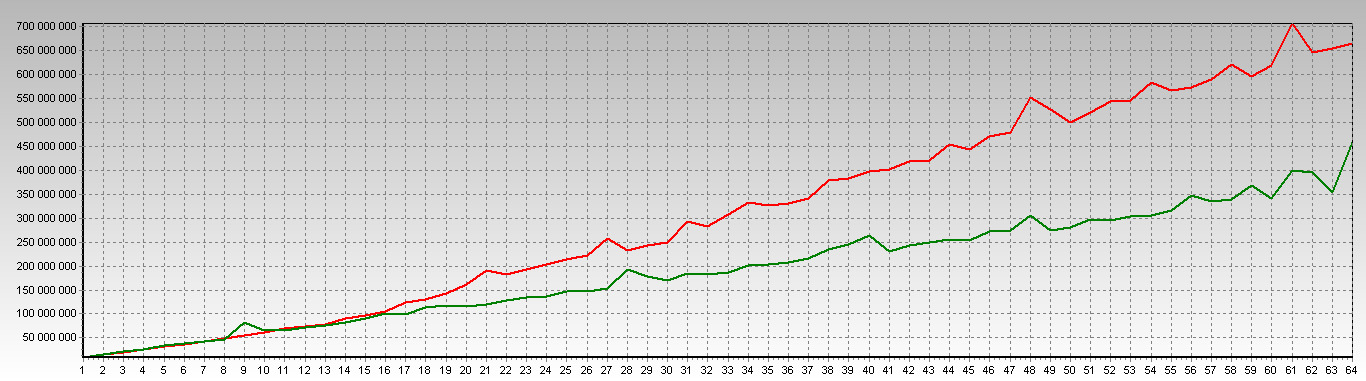
\includegraphics[scale=0.3]{img/read.jpg}
	\end{center}
	\captionsetup{justification=centering}
	\caption{Исследование оптимизирующих структур данных}
	\label{img:read}
\end{figure}

\section{Результаты эксперимента}

В результате исследования оптимизирующих структур данных, показанном на рисунке \ref{img:read_result}, получено, что неоптимизированная структура обрабатывалась в 1,6132398 раз дольше.

\begin{figure}[H]
	\begin{center}
		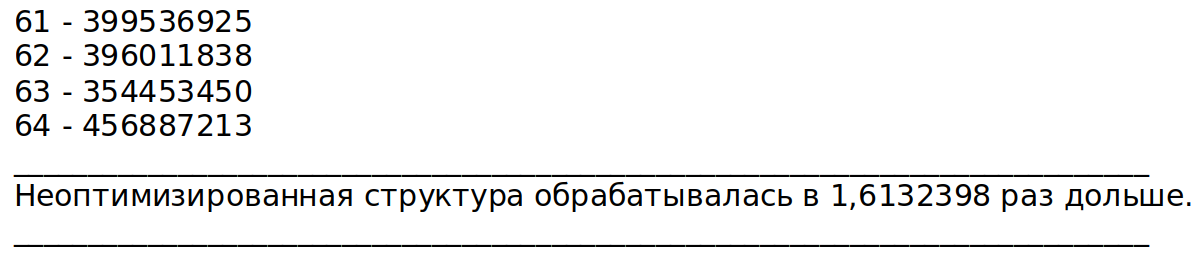
\includegraphics[scale=0.4]{img/read_result.png}
	\end{center}
	\captionsetup{justification=centering}
	\caption{Результат исследования оптимизирующих структур данных}
	\label{img:read_result}
\end{figure}

\section{Вывод}

Для ускорения работы алгоритмов, необходимо правильно упорядочить данные.

\chapter{Эксперимент «Исследование конфликтов в кэш-памяти»}

Цель эксперимента заключается в исследовании влияния конфликтов кэш-памяти на эффективность вычислений.

\section{Исходные данные}

\begin{itemize}
	\item размер банка кэш-памяти данных первого и второго уровня;
	\item степень ассоциативности кэш-памяти первого и второго уровня;
	\item размер линейки кэш-памяти первого и второго уровня.
\end{itemize}

\section{Настраиваемые параметры}

\begin{itemize}
	\item размер банка кэш-памяти, равный 256;
	\item количество читаемых линеек, равное 32;
	\item размер линейки кэш-памяти, равный 64.
\end{itemize}

\section{Графики полученных характеристик}

На рисунке \ref{img:conflict} красный график (верхний) показывает количество тактов работы процедуры, читающей данные с конфликтами в кэш-памяти. Зеленый график (нижний) показывает количество тактов работы процедуры, не вызывающей конфликтов в кэш-памяти. Ось абсцисс отражает смещение читаемой ячейки от начала блока данных. Ось ординат отображает количество тактов.

\begin{figure}[H]
	\begin{center}
		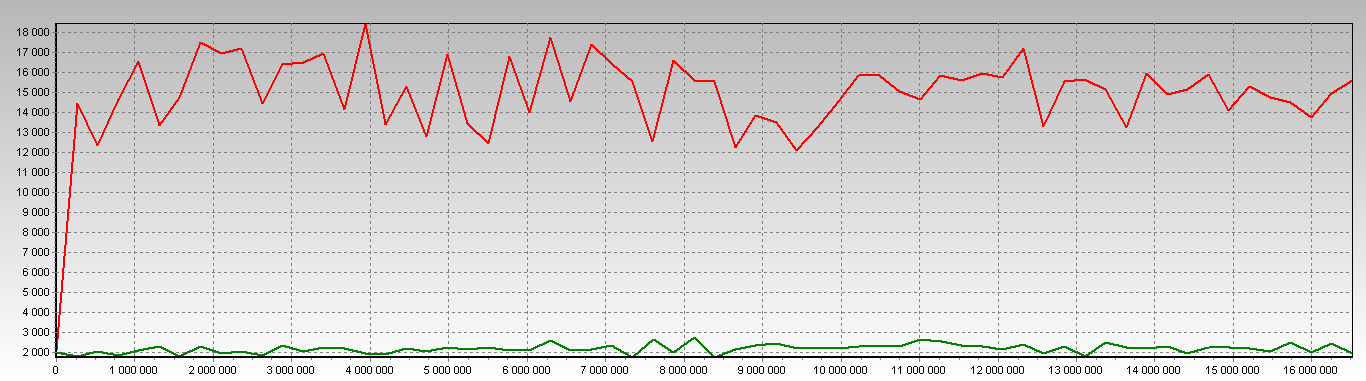
\includegraphics[scale=0.3]{img/conflict.jpg}
	\end{center}
	\captionsetup{justification=centering}
	\caption{Исследование конфликтов в кэш-памяти}
	\label{img:conflict}
\end{figure}

\section{Результаты эксперимента}

В результате исследования конфликтов в кэш-памяти, показанном на рисунке \ref{img:conflict_result}, получено, что чтение с конфликтами банков производилось в 6,7962867 раз дольше.

\begin{figure}[H]
	\begin{center}
		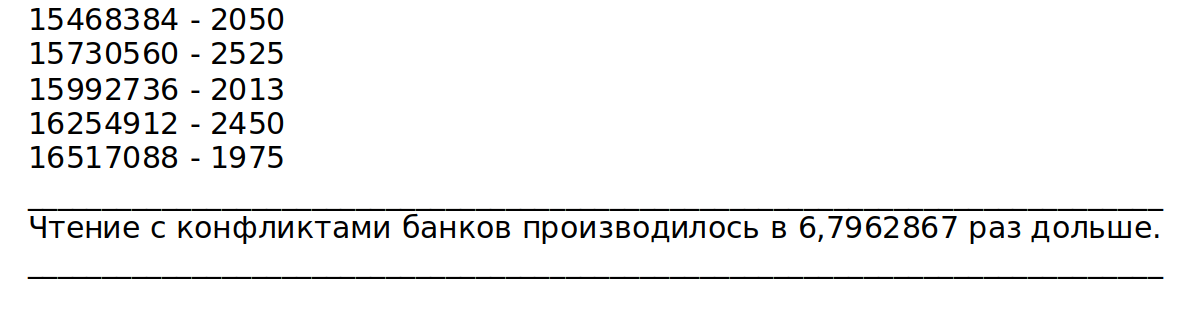
\includegraphics[scale=0.4]{img/conflict_result.png}
	\end{center}
	\captionsetup{justification=centering}
	\caption{Результат исследования конфликтов в кэш-памяти}
	\label{img:conflict_result}
\end{figure}

\section{Вывод}

Использование кэш-памяти ускоряет работу процессора почти в 7 раз.

\chapter{Эксперимент «Исследование алгоритмов сортировки»}

Цель эксперимента заключается в исследовании способов эффективного использования памяти и выявлении наиболее эффективных алгоритмов сортировки, применимых в вычислительных
системах.

\section{Исходные данные}

\begin{itemize}
	\item количество процессоров вычислительной системы;
	\item размер пакета;
	\item количество элементов в массиве;
	\item разрядность элементов массива.
\end{itemize}

\section{Настраиваемые параметры}

\begin{itemize}
	\item количество 64-х разрядных элементов массивов, равное 10;
	\item шаг увеличения размера массива, равный 1024.
\end{itemize}

\section{Графики полученных характеристик}

На рисунке \ref{img:sort} синий график (верхний) показывает количество тактов работы алгоритма QuickSort. Красный график (средний) показывает количество тактов работы неоптимизированного алгоритма Radix-Counting. Зеленый график (нижний) показывает количество тактов работы оптимизированного под 8-процессорную вычислительную систему алгоритма Radix-Counting. Ось абсцисс отражает количество 64-разрядных элементов сортируемых массивов. Ось ординат отображает количество тактов.

\begin{figure}[H]
	\begin{center}
		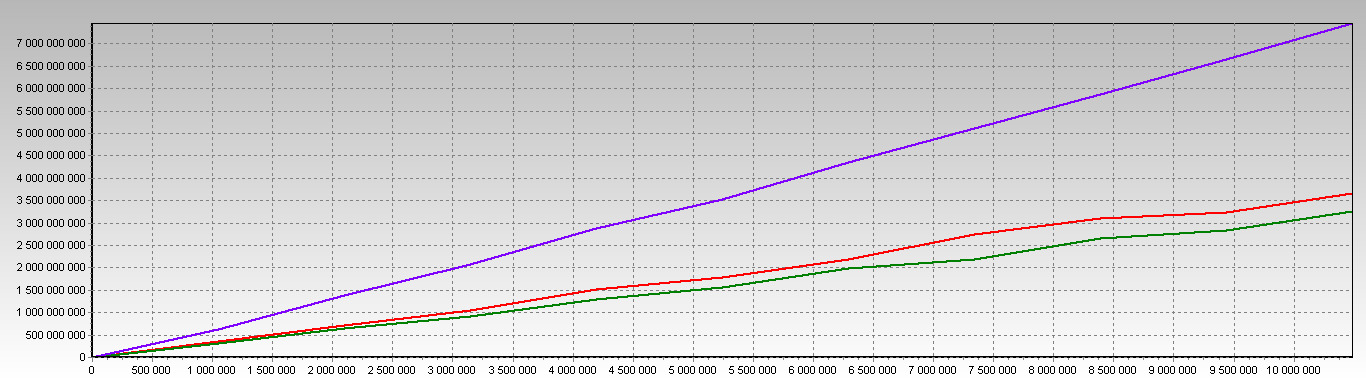
\includegraphics[scale=0.3]{img/sort.jpg}
	\end{center}
	\captionsetup{justification=centering}
	\caption{Исследование алгоритмов сортировки}
	\label{img:sort}
\end{figure}

\section{Результаты эксперимента}

В результате сравнения времени работы алгоритмов сортировки, показанном на рисунке \ref{img:sort_result}, получено, что QuickSort работал в 1,963879 раз дольше Radix-Counting Sort, и 
QuickSort работал в 2,2629607 раз дольше Radix-Counting Sort, оптимизированного под 8-процессорную ЭВМ.

\begin{figure}[H]
	\begin{center}
		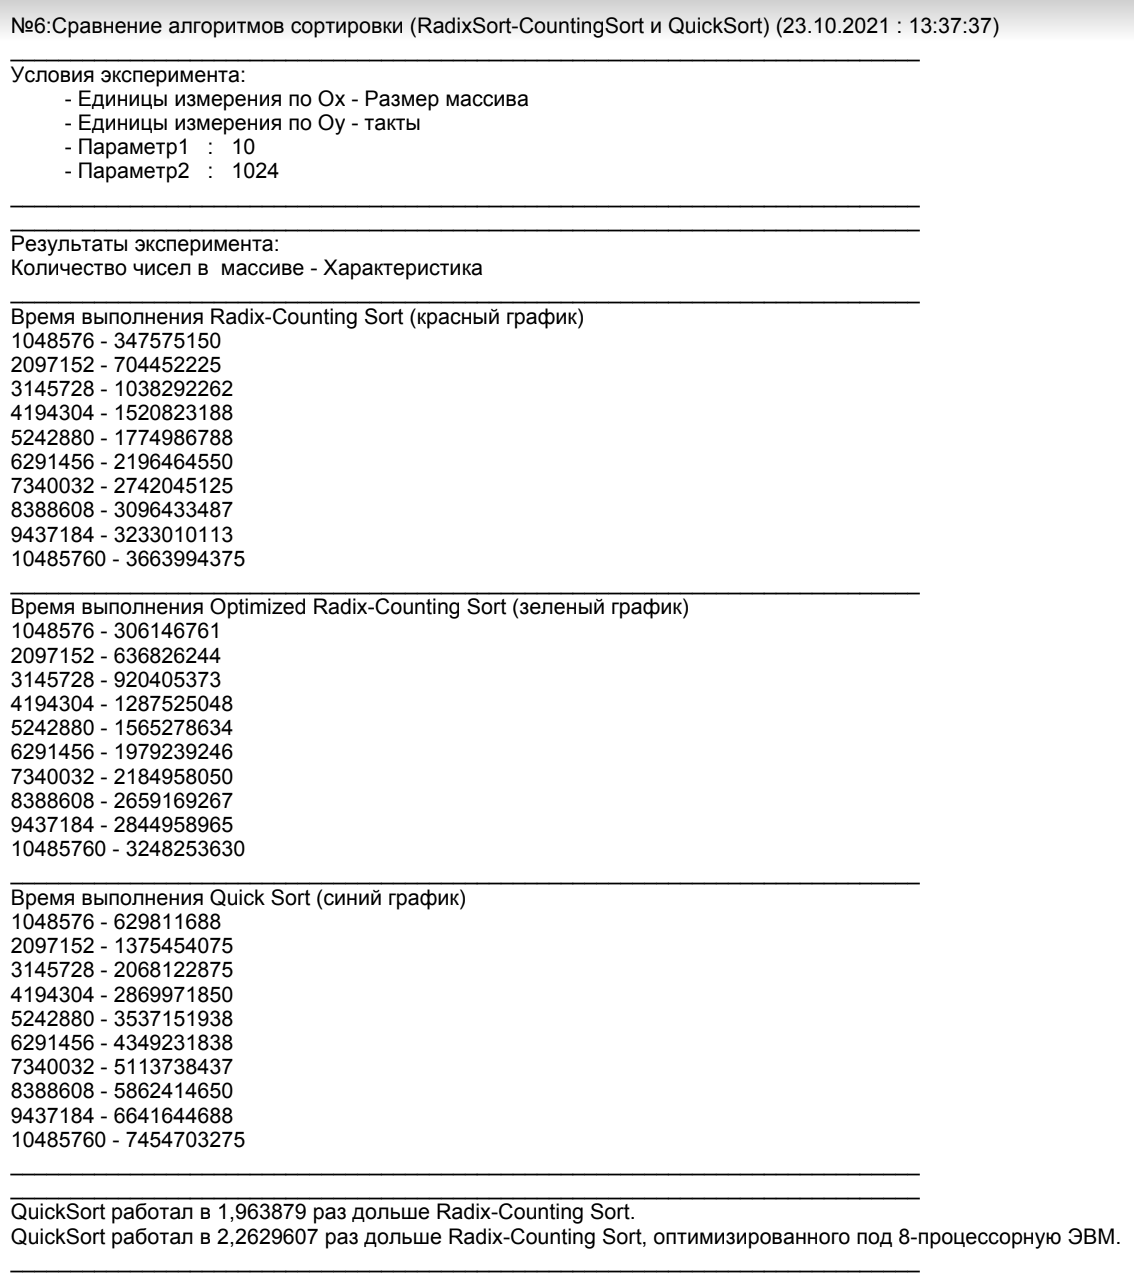
\includegraphics[scale=0.4]{img/sort_result.png}
	\end{center}
	\captionsetup{justification=centering}
	\caption{Результат сравнения времени работы}
	\label{img:sort_result}
\end{figure}

\section{Вывод}

Radix-Counting Sort является более быстрой сортировкой, чем QuickSort, при этом Radix-Counting Sort можно улучшить, оптимизировав алгоритм под 8-процессорную ЭВМ.

\chapter{Контрольные вопросы}

\textbf{1. Назовите причины расслоения оперативной памяти.}

Причиной расслоения оперативной памяти является дисбаланс в скорости доступа к данным, размещенным в оперативной памяти, и производительностью процессора.

\textbf{2. Как в современных процессорах реализована аппаратная предвыборка?}

Аппаратная предвыборка происходит без участия программиста или компилятора. Кэш-контроллер анализирует, по каким адресам и в каком порядке программа обращается к оперативной памяти, и пытается предугадать, какие данные вскоре могут понадобиться программе, и осуществляет их автоматическую предвыборку в кэш-память.

\textbf{3. Какая информация храниться в TLB?}

TLB (Translation-Lookaside Buffer) представляет собой память с ассоциативной выборкой, которая содержит 20-тиразрядные базовые адреса 32-х страниц, то есть, старшие 20 разрядов физического адреса страницы.

Каждый из базовых адресов имеет свой признак - тег. В качестве тега используются старшие 20 разрядов линейного адреса, то есть поля TABLE и PAGE.

Помимо тега для каждого базового адреса страницы в TLB хранится
дополнительная информация, позволяющая определить, какую страницу можно заменить на вновь вводимую.

\textbf{4. Какой тип ассоциативной памяти используется в кэш-памяти второго уровня
современных ЭВМ и почему?}

В современных компьютерах применяют кэш-память второго уровня,
которая находится между процессором и оперативной памятью и еще больше повышает производительность ЭВМ, потому что кэш-память 2-го уровня, может содержать как команды, так и данные.

\textbf{5. Приведите пример программной предвыборки.}

Примерами программной предвыборки являются предвыборка данных в цикле для независимости от информации находящейся вне цикла и предвыборка в основных блоках, которые часто исполняются, но которые редко используют ее независимо от целей предвыборки.